
%%%%%%%%%%%%%%%%%%%%%%%%%%%%%%%%%%%%%%%%%%%%%%%%%%%%%%%%%%%%%%%%%%%%%
%% This is a (brief) model paper using the achemso class
%% The document class accepts keyval options, which should include
%% the target journal and optionally the manuscript type.
%%%%%%%%%%%%%%%%%%%%%%%%%%%%%%%%%%%%%%%%%%%%%%%%%%%%%%%%%%%%%%%%%%%%%
\documentclass[journal=jacsat,manuscript=article]{achemso}

%%%%%%%%%%%%%%%%%%%%%%%%%%%%%%%%%%%%%%%%%%%%%%%%%%%%%%%%%%%%%%%%%%%%%
%% Place any additional packages needed here.  Only include packages
%% which are essential, to avoid problems later. Do NOT use any
%% packages which require e-TeX (for example etoolbox): the e-TeX
%% extensions are not currently available on the ACS conversion
%% servers.
%%%%%%%%%%%%%%%%%%%%%%%%%%%%%%%%%%%%%%%%%%%%%%%%%%%%%%%%%%%%%%%%%%%%%
\usepackage[version=3]{mhchem} % Formula subscripts using \ce{}
\usepackage[T1]{fontenc}       % Use modern font encodings

%%%%%%%%%%%%%%%%%%%%%%%%%%%%%%%%%%%%%%%%%%%%%%%%%%%%%%%%%%%%%%%%%%%%%
%% If issues arise when submitting your manuscript, you may want to
%% un-comment the next line.  This provides information on the
%% version of every file you have used.
%%%%%%%%%%%%%%%%%%%%%%%%%%%%%%%%%%%%%%%%%%%%%%%%%%%%%%%%%%%%%%%%%%%%%
%%\listfiles

%%%%%%%%%%%%%%%%%%%%%%%%%%%%%%%%%%%%%%%%%%%%%%%%%%%%%%%%%%%%%%%%%%%%%
%% Place any additional macros here.  Please use \newcommand* where
%% possible, and avoid layout-changing macros (which are not used
%% when typesetting).
%%%%%%%%%%%%%%%%%%%%%%%%%%%%%%%%%%%%%%%%%%%%%%%%%%%%%%%%%%%%%%%%%%%%%
\newcommand*\mycommand[1]{\texttt{\emph{#1}}}
\usepackage{color}
\def\todo#1{{\color{red}[TODO: #1]}}
\def\added#1{{\color{blue} #1}}
\def\removed#1{{\color{magenta}[Removed: #1]}}
\def\note#1{{\color{cyan}[Note on edit: #1]}}

%%%%%%%%%%%%%%%%%%%%%%%%%%%%%%%%%%%%%%%%%%%%%%%%%%%%%%%%%%%%%%%%%%%%%
%% Meta-data block
%% ---------------
%% Each author should be given as a separate \author command.
%%
%% Corresponding authors should have an e-mail given after the author
%% name as an \email command. Phone and fax numbers can be given
%% using \phone and \fax, respectively; this information is optional.
%%
%% The affiliation of authors is given after the authors; each
%% \affiliation command applies to all preceding authors not already
%% assigned an affiliation.
%%
%% The affiliation takes an option argument for the short name.  This
%% will typically be something like "University of Somewhere".
%%
%% The \altaffiliation macro should be used for new address, etc.
%% On the other hand, \alsoaffiliation is used on a per author basis
%% when authors are associated with multiple institutions.
%%%%%%%%%%%%%%%%%%%%%%%%%%%%%%%%%%%%%%%%%%%%%%%%%%%%%%%%%%%%%%%%%%%%%

\author{Robert O. Ness}
\affiliation[Purdue University]{Purdue University Department of Statistics, West Lafayette}
\alsoaffiliation[Northeastern University]{College of Science, College of Computer and Information Science, Northeastern University, Boston}
\affiliation[Northeastern University]{College of Science, College of Computer and Information Science, Northeastern University, Boston}
\author{Karen Sachs}
\affiliation[Stanford University]{School of Medicine, Stanford University, Palo Alto}
\author{Olga Vitek}
\email{o.vitek@neu.edu}
\affiliation[Northeastern University]{College of Science, College of Computer and Information Science, Northeastern University, Boston}



%%%%%%%%%%%%%%%%%%%%%%%%%%%%%%%%%%%%%%%%%%%%%%%%%%%%%%%%%%%%%%%%%%%%%
%% The document title should be given as usual. Some journals require
%% a running title from the author: this should be supplied as an
%% optional argument to \title.
%%%%%%%%%%%%%%%%%%%%%%%%%%%%%%%%%%%%%%%%%%%%%%%%%%%%%%%%%%%%%%%%%%%%%
 \title[]
   {From correlation to causality: statistical approaches to learning regulatory relationships in large-scale biomolecular investigations}

%%%%%%%%%%%%%%%%%%%%%%%%%%%%%%%%%%%%%%%%%%%%%%%%%%%%%%%%%%%%%%%%%%%%%
%% Some journals require a list of abbreviations or keywords to be
%% supplied. These should be set up here, and will be printed after
%% the title and author information, if needed.
%%%%%%%%%%%%%%%%%%%%%%%%%%%%%%%%%%%%%%%%%%%%%%%%%%%%%%%%%%%%%%%%%%%%%
\abbreviations{IR,NMR,UV}
\keywords{causal inference, big data, causal networks, Bayesian networks}

%%%%%%%%%%%%%%%%%%%%%%%%%%%%%%%%%%%%%%%%%%%%%%%%%%%%%%%%%%%%%%%%%%%%%
%% The manuscript does not need to include \maketitle, which is
%% executed automatically.
%%%%%%%%%%%%%%%%%%%%%%%%%%%%%%%%%%%%%%%%%%%%%%%%%%%%%%%%%%%%%%%%%%%%%
\begin{document}

\begin{abstract}
  Causal inference -- the task of uncovering regulatory relationships between components of biomolecular pathways and networks - is a primary goal of many high throughput investigations.  Statistical associations between quantitative measurements can suggest an enticing number of hypotheses regarding the underlying causal interactions. But when do such associations reflect the underlying causal biomolecular mechanisms?  The goal of this perspective is to provide suggestions for causal inference in large scale experiments, which utilize high throughput technologies such as mass spectrometry-based proteomics.  We describe in non-technical terms the pitfalls of inference in large datasets, and suggest methods to overcome these pitfalls and reliably find regulatory associations.
\end{abstract}

%%%%%%%%%%%%%%%%%%%%%%%%%%%%%%%%%%%%%%%%%%%%%%%%%%%%%%%%%%%%%%%%%%%%%
%% Start the main part of the manuscript here.
%%%%%%%%%%%%%%%%%%%%%%%%%%%%%%%%%%%%%%%%%%%%%%%%%%%%%%%%%%%%%%%%%%%%%
\section{Introduction}

%\note{Olga's comment: Modern experiments generate large scale data
%Correlation. Not enough. Causal inference elucidates.... or causal relationships  Examples are XXX However this is difficult because XXX}

\added{Modern high-throughput technologies such as mass spectrometry simultaneously quantify hundreds or even thousands of biomolecular analytes.  Statistical associations (e.g. Pearson correlation, Spearman correlation, and mutual information) between the analytes  can suggest an enticing number of hypotheses regarding the underlying causal biomolecular mechanism.  However, associations do not imply causation. Formal methods of causal inference \cite{pearl2009causality,markowetz2007inferring} are required to probe these statistical associations for causality, and infer the underlying regulatory mechanisms. }

\added{There is an increasing interest in causal inference in proteome research. It has previously been used to learn the directed structure of signal transduction networks, e.g. in flow cytometry investigations in Sachs et al. 2005 \cite{sachs2013single}, antibody/bead-based XMAP technology from Luminex in Saez-Rodriguez et al. 2009\cite{saez2009discrete} and participants in the DREAM4 Predictive Signaling Network Challenge\cite{prill2011crowdsourcing}.
However, the successful examples of causal inference in proteomics are very few \cite{bensimon2012mass}. In this perspective we demonstrate that this is not an accident.  The difficulty stems from the fact that large numbers of quantified analytes, combined with small sample size, lead to more spurious pairwise associations, obfuscate the true signal, and increase the false discoveries of putative causal events. Below we describe in non-technical terms the process of elucidating causal associations from high-throughput data, and suggest practical approaches for causal inference in large scale proteomic datasets.  Specifically, we suggest that the task of causal inference can be facilitated by refining the biological question, and by improving experimental design in terms of selection of  (1) the subset of analytes, (2) the number of biological replicates, and (3) the type of biological conditions and stresses. }


\section{I. Small-scale statistical inference of causal relationships: conditional independence and interventions}

\begin{figure}[!tpb]
\centerline{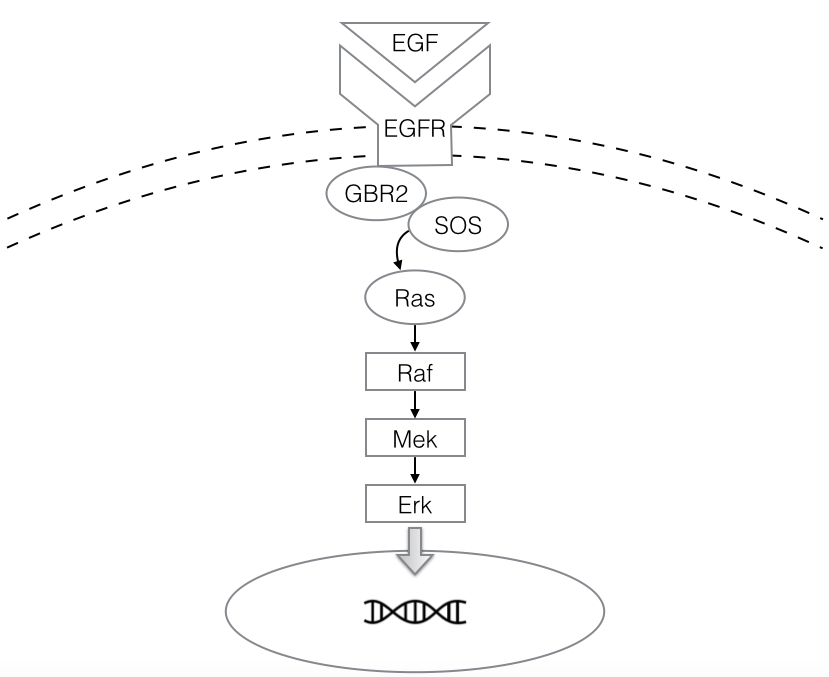
\includegraphics[width=.5\textwidth]{figs/egfr.png}}
\caption{EGFR MAPK signaling pathway, an example of a pathway containing the phosphorylation cascade from Raf to Mek to Erk.  The binding of ligand EGF to EGFR initiates a signal that leads to the cascade, which in turn regulates transcription.  This cascade implies two direct causal relationships, namely Raf --> MEK, and Mek --> Erk.  Raf and Erk have an indirect causal relationship, through Mek.\label{mapk}}
\end{figure}

Consider, e.g. the MAPK signaling cascade in Figure \ref{mapk}, which is part of several signaling pathways such as the EGFR MAPK pathway\cite{holbro2004erbb}. In this cascade Raf causally affects the level of active (i.e., phosphorylated) Mek, while Mek causally affects Erk. Imagine these causal relationships were unknown: could they be detected from quantitative measurements on these phosphoproteins?  

To illustrate the process of causal inference in this context, we simulated artificial data using the computational Huang-Ferrell model \cite{huang1996ultrasensitivity} of this cascade. The model represents the key binding, phosphorylation, and dephosphorylation reactions of the cascade with mass action kinetics, and replicates the MAPK key signaling behavior observed in nature.  We used the model to simulate an experiment with 50 replicate biological samples, and measurements of concentration (umol) of phosphorylated Raf, and doubly phosphorylated Mek and Erk in each sample. 

\begin{figure}[!tpb]
\centerline{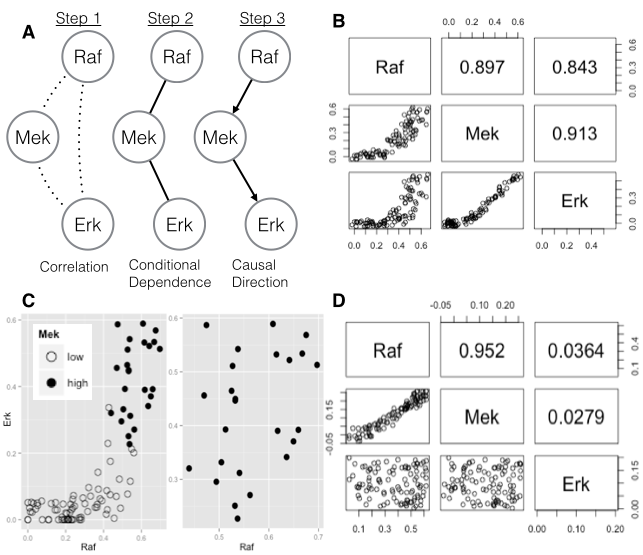
\includegraphics[width=.95\textwidth]{figs/mapk.png}}
\caption{A: Overview of the 3 steps of causal inference, illustrated for the MAPK signaling cascade.    B, C, and D feature an experiment simulated from the Huang-Ferrell computational model of the phosphorylation cascade.  B: Pairwise plots of concentration values of phosphorylated (doubly phosphorylated for Mek and Erk) forms of each protein, and observed Spearman correlation values.  The Raf -- Erk correlation is high, despite the fact that Raf does not directly regulate Erk.  C: Concentrations of Raf versus Erk, where samples corresponding to high Mek (here, set to the top quartile) are highlighted \added{with filled circles}.  The right panel of C shows the subset of samples with high Mek (i.e. conditional on Mek being high). In these samples the association between Raf and Erk disappears, \added{and we infer} that Raf and Erk are {\it conditionally independent} given Mek.  D:  After Mek is inhibited, the observed association between Raf and Mek remains, while the association between Mek and Erk disappears. This reveals the causal flow from Raf to Mek. 
\label{mapkInference}}
\end{figure}


Figure \ref{mapkInference}A demonstrates the causal inference workflow starting with analysis of statistical associations in the data.  In step 1, a correlation graph between cascade components Raf, Mek, and Erk is assembled from the measurements of protein concentration.  Step 2 reduces the correlation graph to a \added{sparse graph of inferred} underlying conditional dependencies (Raf--Mek, and Mek--Erk).  Step 3 interrogates this graph to find putative directions of causal relationships (Raf-->Mek, and Mek-->Erk).  While step 1 has little requirements, step 2 requires multiple samples or replicates, and step 3 requires systematic interventions (e.g. with protein inhibitors). 

Figure \ref{mapkInference}B illustrates Step 1 of the causal inference, and shows 2-way plots of the protein concentrations across the biological samples, and Spearman correlations to quantify the extent of the associations. \added{We chose Spearman correlation instead of Pearson correlation because it best quantifies nonlinear relationships.}  The correlation values are high, and would meet most reasonable cut-off thresholds for constructing the correlation network in the left part of panel A.  The Raf--Mek and the Mek--Erk correlation edges match the Raf-->Mek, Mek-->Erk known causal edges.  What about the non-causal Raf--Erk edge? Despite the high Raf--Erk correlation, there is no direct causal mechanism between them (aside from the one via Mek, which is already accounted for via the Raf-->Mek and Mek-->Erk edges).  In causal  inference, our goal is to eliminate this ``nuisance" edge.  How is this done?

\added{To describe Step 2 of causal inference, we introduce some terminology. If concentrations of two proteins vary between the biological samples in a coordinated manner, such that knowing the concentration of one protein provides information on the concentration of the other, the two proteins are called {\it dependent}. Otherwise they are called {\it independent}. {\it Conditional independence} is a special case that is important to causal inference.  Two {\it dependent} proteins are {\it conditionally independent} if, after knowing (in probability language, {\it conditioning on}) the concentration of third-party biomolecules, the two proteins become independent. In other words, after considering the information from the third party, the behavior of one protein provides no additional information on the behavior of the other.}. 

\added{While statistical associations and correlations are properties of the observed data, dependence and conditional independence are properties of the underlying processes that generate the data. Step 2 relies on statistical inference\cite{pearl2009causality,markowetz2007inferring} to infer from the observed data pairs of proteins that are conditionally independent. The conditionally independent pairs are ignored, and the remaining pairs are kept as hypothesized causal relations. This sparse inferred conditional independence graph is often desirable, as it reduces the many pairwise associations to a smaller number of hypothesized causal relations.}

Let's see how this applies to the MAPK signaling cascade. \added{Since Raf regulates the concentration of Erk by way of regulating Mek, Raf and Erk are dependent.  However, if we know the concentration of Mek, then the concentration of Raf provides no additional information about the concentration of Erk. Therefore, even though Raf and Erk are dependent, they are also conditionally independent given Mek.  }  Figure \ref{mapkInference}C illustrates the process of statistical inference by comparing the concentrations of Raf and Erk. When we subset the measurements to only the samples with high Mek, we can no longer see the association between Raf and Erk. \added{Formally, the algorithm tests the null hypothesis of conditional independence between Raf and Erk given the full range of values of Mek (and not just high values of Mek, as was shown for the purposes of illustration), and evaluates evidence against the null hypothesis\cite{spirtes2000causation}. In this example the test did not reject the null hypothesis, and resulted in removing the edge between Raf and Erk as in the middle graph of Figure \ref{mapk}A. }

At Step 2 the direction of the regulation remains unknown. Inference of the direction of the chain of events requires the experimental design, which involves external interventions or stresses. Figure \ref{mapkInference}D illustrates the results of Step 3, in the case where an intervention targeted Mek with an inhibitor. The intervention does not affect the concentration of Mek, however it blocks its ability to phosphorylate other proteins.  After this intervention the Raf--Mek relationship is unchanged, while Erk drops to a low level.  From this we can infer that Mek has causal influence on Erk. Since Raf was unaffected by the intervention, Mek does not have a causal influence on Raf, and therefore the direction of causal influence in this edge goes from Raf to Mek.  This intervention is required to transform the undirected graph in panel A - Step 2 to the causal graph in panel A - Step 3.

In the general case, computational methods for causal inference follow the workflow in Figure \ref{mapkInference}A, while scaling it to characterize multiple inter-related proteins. Step 1 creates a dense network of pairwise associations. \added{Step 2 identifies cases of conditional independence, and removes the corresponding edges to create a much sparser network.}  Finally, Step 3 uses the experimental design, specifically the information regarding the interventions, to evaluate these edges as evidence for potential causal events. See Koller and Friedman \cite{koller2009probabilistic} for a detailed description of these methods and their theoretical underpinnings. Numerous implementations are available in statistical software, e.g. in the R package {\tt bnlearn} \cite{scutari2009learning}. \added{Depending on the biological system and on the experimental setting, the strength of causal evidence may vary. For example, Sachs, Itani {\it et al.} 2013\cite{sachs2013single} highlight conditions in phosho-proteomic experiments  where it may be infeasible to disentangle causality using perturbations.} 


%%%%%%%%%%%%%%%%%%%%%%%%%%%%%%%%%%%%%%%%%%%%%%%%%%%%%%%%%%%%%%%%%%%%%%%%%%%%%%%%%%%%%%%%%%%%%%%
\section{II. Large-scale statistical inference of causal relationships: challenges of scaling up}

\added{Experimentalists can choose to quantify more or less analytes, and collect more or less replicates such as proteins.} A typical high-throughput experiment includes \removed{a small number of interventions,} a small number of biological replicates, and quantifies a large number of analytes \removed{such as proteins}. \removed{This creates challenges in each of the 3 steps of causal inference above.}  \added{This experimental approach is an obstacle to causal inference.}

\added{To understand why, recall that we are interested in paring down the correlation graph in step 1 to the sparse conditional independence graph in step 2.}  In Step 1, the challenge is in quantifying statistical associations between each pair of the analytes across the biological samples. A large number of analytes yields a large number of spurious statistical associations, which arise without any biological justification, and are purely an artifact of random chance. Systematic pairwise relationships such as between Raf, Mek and Erk in the MAPK pathway will be obscured by the many spurious relationships that they will each form with causally unrelated proteins.

We illustrate this problem with a computer simulation, inspired by Fan et. al\cite{fan2014challenges} but translated to our context. First, we simulated an experiment that quantifies the abundances of 60 proteins in 60 biological samples. Second, we simulated another experiment where the number of proteins was increased from 60 to 6000. In both experiments the proteins are completely independent from each other, and each protein in each replicate is assigned a value randomly drawn from a Gaussian distribution. In other words, we do not expect any biologically meaningful associations in these data. We repeated each of these simulations 500 times. Figure \ref{spur_corr} shows for each experiment the histogram of the highest Pearson correlation across any pair of proteins in the 500 instances of the simulation. As can be seen, the increase to 6000 proteins produces relatively large maximum pairwise correlations, demonstrating that an increase in the number of proteins leads to an increase in spurious correlation.  This is clearly a problem when high Pearson correlation is used as an initial evidence of biological function.

\begin{figure}[!tpb]
\centerline{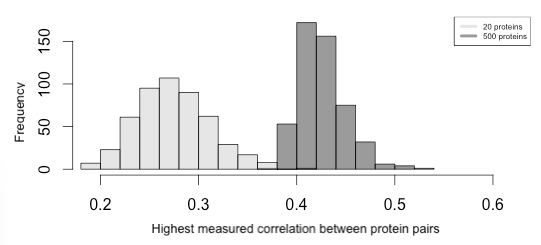
\includegraphics[width=.8\textwidth]{figs/spurious_corr.png}}
\caption{Histogram of maximum observed correlation values between unrelated protein pairs in a simulation of 500 experiments.  In each iteration,  first 60 proteins are quantified, after which throughput is increased to 6000 proteins.  Increasing the number of proteins increases spurious correlation.  This is a problem because correlation is used as initial evidence for a biological relationship.}
\label{spur_corr}
\end{figure}

Similarly, the increased incidence of spurious correlations impedes the performance of statistical methods in Step 2, which elucidate conditional independences in the data.  If we think of this step as \added{attempting to detect which pairs are not conditionally independent}, then the spurious correlations result in more false positives \added{detections}. To illustrate, \added{we performed a second simulation}, this time we included some dependence between proteins so we could evaluate the effect of dimensionality of the data on true positives (pairs of proteins that are not conditionally independent) as well as false positives.  

\added{To build dependence into the simulated data, we created multiple sets of 3-proteins "triplets" A, B, and C, where all three are dependent but A and B are conditionally independent given C.  Thus perform perfectly on the $i^{th}$ triplet, the algorithm would need two true positives (rejecting conditional independence between $A_i$ -- $C_i$ and $B_i$ -- $C_i$), find the $A_i$ and $B_i$ pair conditionally independent, and find any pair containing a node in the $i^th$ triplet and any node not in the $i^{th}$ triplet to be independent.  We made it such that the proteins in each triplet generate measurements with Gaussian values with mean 0 and variance 1, and that the covariance between A--C and B--C was .3.  We simulated data from a multivariate Gaussian. }

\added{Again we run the simulation 500 times, in each iteration we performed step 1 by calculating pairwise Pearson correlations, and then Step 2 by applying the Grow-Shrink algorithm \cite{margaritis2003learning} for causal inference, an instance from a class of algorithms called constraint-based network inference algorithms\cite{spirtes2000causation} that proceed with a series of conditional independence tests that control the false positive rate.  To assure we weren't observing algorithm specific effects, we also repeated the simulation other algorithms from this class\cite{tsamardinos2003algorithms}\cite{yaramakala2005speculative} .  The results did not differ (results not shown).}  

\added{These algorithms have stricter data requirements that correlation calculations, so in this simulation we increase from 60 proteins to only 99.  The starting 60 proteins contains 20 triplets, and thus perfect performance of the algorithm would yield 40 true positives (and of course 0 false positives).  In a high-throughput experiment, the investigator may arbitrarily select proteins for quantification, hoping the more proteins are quantified, the higher the chance of uncovering biology.  Alternatively, he or she may apply their prior knowledge about the system to select proteins that are strong candidates for being involved in the biology.  We respectively term these approaches "uninformed addition" and "informed addition" of proteins.  We simulate "uniformed addition" but adding 39 proteins to the original 60 that are completely independent.  In this case perfect performance is still 40 true positives.  In the second "informed addition" case, we add 13 new triplets, increasing the perfect performance standard from 40 to 66.  In addition to comparing these two strategies, we compare the 60 replicate case to the 100 replicate case, to show what role sample size has in affecting performance.}

Figure \ref{spur_dep} shows the counts of false positive edges in the resulting conditional independence graph, i.e. the number of protein pairs \added{where the null hypothesis of conditional independence was unduly rejected}.  The results demonstrate that an increase in the number of proteins leads to an increase in false positive rejections of conditional independence, and to a denser conditional independence graph.  \added{This occurs because the number of false positives depends on the total number of pairwise comparison -- a 65\% increase from 60 to 99 proteins results in a 175\% increase in the number of comparisons.  In other words, the computational methods for causal inference are more likely to fail in a large-scale experiment, because they cannot reliably distinguish the potential causal relationships from noise.}

\begin{figure}[!tpb]
\centerline{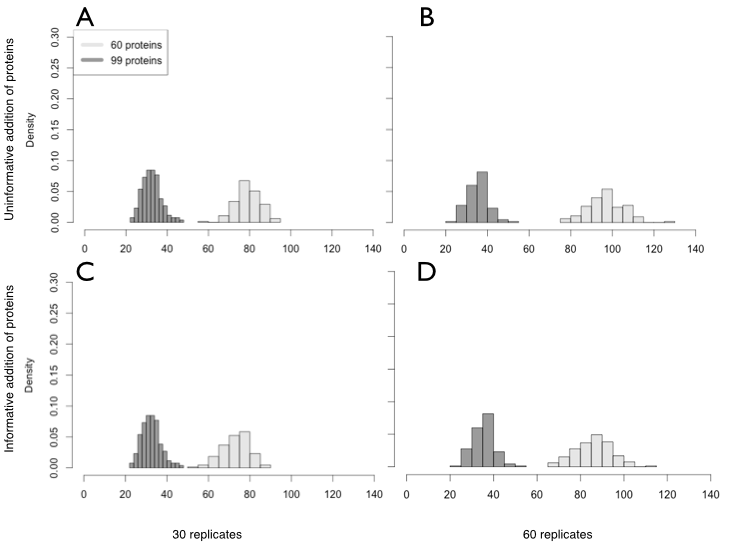
\includegraphics[width=.8\textwidth]{figs/spurious_dep2.png}}
\caption{Histograms of false positives detection of relationships between proteins (rejections of tests for conditional independence) over 500 simulated experiment.  Simulated experiments start with quantifying 60 and then expand to 99.  The initial 60 proteins contains 40 pairwise relationships that the algorithm is based with detection.  In parts A and B, 39 proteins are added that have no relationship with any other protein.  In parts C and D, 39 proteins are added that have 26 additional pairwise relationships. The left column parts A and C show results with 60 replicates, the right column B and D for 100 replicates.  Increasing the number of proteins results in more false positives without any biological justification.  Informed addition of proteins mitigates this only slightly.  Adding replicates paradoxically increases false positives.  In both cases there are less replicates than pairwise comparisons, so the extra replicates add degrees of freedom which enables more tests, some of which add to the total false positives.}
\label{spur_dep}
\end{figure}

\added{Comparing the panels figure \ref{spur_dep} reveals a noteworthy result; informed addition of proteins offers only a slight reduction in false positives on average.  Increasing sample size doesn't help much either, paradoxically in this case it hurt, because even at 100 replicates there are still  more pairwise comparisons than replicates, so the algorithm uses every last degree of freedom at its disposal.  Increasing the number of replicates from 60 to 100 therefore allowed more conditional independence tests to take place, and some of these additional tests added to the false positive count.} 

\begin{figure}[!tpb]
\centerline{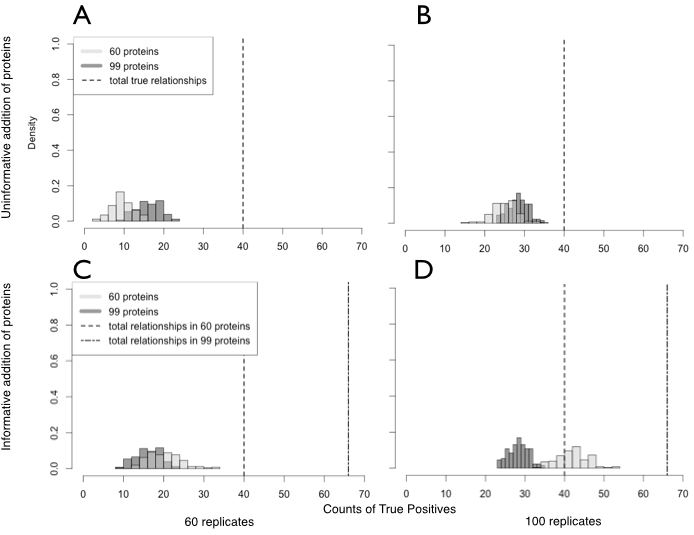
\includegraphics[width=.8\textwidth]{figs/true_pos.png}}
\caption{Simulated experiments quantifying 60 and 99 unrelated proteins in 60 and 100 biological samples. The histograms display the counts of true positives in conditional independence tests between pairs of proteins, calculated over 500 repetitions of the simulation. The top row parts A and B illustrate uninformed addition of 39 proteins to the starting amount of 60, the bottom parts C and D illustrate informed addition.  The left column parts A and C show results with 60 replicates, the right column B and D for 100 replicates.  Dashed lines indicate the total amount of positives the algorithm is tasked with discovering.  Increasing the number of replicates increases true positives and is indeed essential when increasing the number of proteins increases the number of relationships to be detected.}
\label{true_pos}
\end{figure}

\added{So what exactly is the use of having more replicates? How does an informed selection of proteins for the panel make a difference relative to random selection?  These factors come to play in detection of true positives.  Figure \ref{true_pos} is the true positive counterpart to figure\ref{spur_dep}.  Parts A and B illustrate the 40 true positives upper bound on performance with the dashed line, and in parts C and D, where "informed addition" of proteins is applied, the increase upper bound of 66 is pictured with the double-dashed line.  Comparing parts A and B show that increasing the number of replicates increases the amount of true positives.  Parts C and D show that when there are more total relationships to detect, having more replicates is essential -- when more relationships were added without increasing replicates, the count of true positives actually decreased slightly on average as the algorithm tries to do more with little.  However, when comparing parts C and D in figure \ref{true_pos} to C and D in figure \ref{spur_dep}, we see that the scale of the increase in total true positives gained from informed addition of proteins was less than that of the increase of false positives.  The spurious correlation and resulting false positives in high throughput experiments quickly outweigh the benefit that informed selection of proteins and greater sample size has on discovery.}

\removed{A related problem with high-throughput experiments in Step 2 is a relatively small number of biological replicates as compared to the number of analytes.  Once again the purpose of step 2 is to test conditional independence, and detect relationships between proteins that remain even when conditioning on other proteins.  While measuring too many analytes causes an explosion in false positives, collecting too few samples results in insufficient power to detect these relationships. While Step 1 (evaluating the set of pairwise associations) can be carried out with even a small amount of replicates, Step 2 relies on having many replicates relative to the number analytes.  Note that even when the experiments demonstrated in Figure 3 had 100 replicates to its 100 proteins, and still false positives were high. The quality of causal inference approaches decreases drastically as the numbers of replicates fall.}

\added{Finally, the challenge of completing step 3 in the workflow also increases with the number of proteins quantified.}  Step 3 requires interventions to infer causal relationships from evidence of conditional independence.  \added{For a panel of k analytes, theoretical work by Eberhardt and Scheines {\it et al.} \cite{eberhardt2012number} show that in least ideal case of the only interventions available being interventions that target a single analyte (such as with small molecule inhibitors), k - 1 separate interventions would be needed.  With application of interventions that simultaneously target multiple analytes, this number can be lowered significantly, but this depends on several different factors\cite{eberhardt2012number,hauser2012two,hyttinen2013experiment} beyond the scope of this discussion.} \removed{For example, in the Raf-Mek-Erk pathway one intervention on Mek was sufficient to infer the two causal relationships. However, scaling this approach to a large number of proteins also introduces.}  But generally speaking as the number of proteins grows, so does the number of interventions required to fully infer causality, and eventually the total number of required interventions may become infeasible. Moreover, if the step 2 results in too many false positive hypothesized causal relations, this will adversely affect the results of step 3 regardless of the size of the dataset.


\section{III. Approaches for inferring causality from high-throughput experiments}

The problems outlined in section II paint a grim picture for causal inference in large datasets. Fortunately, these can be overcome, and effective causal inference can be a reality for large scale datasets.  We provide suggestions for the best practices below.

\begin{enumerate}
\item \textit{Limit the number of analytes.} \added{Reducing the number of analytes dramatically reduces the number of spurious associations and resulting false positives.} Even though a list of analytes quantifiable with high-throughput technologies grows larger, only use a subset of measurements that are both biologically relevant and technologically accurate. The length of the list is not as important as the quality of measurements on the key parts of the system.  If the broader biological system is well understood, it may be possible to design a targeted experiment that focuses on a specific network or pathway, and ask more specific questions of the data, such as the presence of a particular regulatory event.  The more specific the question, the less data are needed to make solid causal conclusions.  

\item \textit{Profile more biological replicates.}  \added{While reducing the number of analytes reduces spurious associations (false positives), increasing the number of replicates increases statistical power (true positives).}  The high-throughput measurements should provide more samples from distinct biological sources, which come from a same underlying population.  This fact gives advantage to technologies, such as targeted proteomics tools, that quantify fewer analytes but have a higher sample throughput.  \added{A review by Twerve and Saez-Rodriguez provides a contrast of technologies by their content and sampling throughput\cite{SaezRodriguez:2012kx}.} 

\added{Single cell mass cytometry is a technology deserving of special mention, where many thousands of cells per sample provide much more data as an input to causal inference, though cell samples still need to be drawn from multiple individuals in order to make inferences about the population from which those individuals were drawn}. See Sachs et al 2005 for an in depth case study of network inference with a single cell dataset. \cite{sachs2005causal}.  

\item \textit{Use prior knowledge.} Prior knowledge improves the search for conditional independence and helps to determine causality. The prior knowledge can be in form of known canonical networks, extracted, e.g. from pathway databases such as KEGG. One example of such prior information is the MAPK pathway. The prior information reduces the search space of unknown associations that need to be considered, enables a more effective use of the data, and increases the confidence in newly discovered statistical associations.  \added{Work by Saez-Rodriguez, Lauffenburger, and Sorger\cite{SaezRodriguez:2009hb}, as well as Terfve and Saez-Rodriguez\cite{Terfve:2015kw} use prior network knowledge to build logic models that reflect causal relationships between signaling proteins using proteomics measurements, the former using antibody/bead-based XMAP technology from Luminex, and the latter using LC-MS/MS.} Another example of prior knowledge is contextual information, such as spatial or temporal annotations of the quantitative measurements in the cell. The contextual information can be extracted from the literature or from other complementary (and potentially noisy) datasets. The causal inference algorithms can be extended to weigh evidence of conditional independence, depending on whether the analytes share the same spatial or temporal context. 

\item \textit{Select targeted interventions wisely.} Targeted interventions perturb individual components of the biological system.  An example is \added{siRNA knockdowns, as well as} small molecule inhibitors, which block the causal influence of a specific protein on its downstream components. Although effective, such targeted interventions are limited in number. Therefore, a strategic experimental design would use prior information, prioritize the interventions and the targets, and apply them to parts of the biological system that have most potential for new discovery of regulatory events.  For example, a graph with undirected edges can be inspected, to reveal which nodes have potential to reveal the most causality if perturbed. Such targeted perturbations can be applied iteratively, after an initial statistical analysis revealed areas of the network where causal inference would benefit from extra measurements and data. 


\item \textit{Consider broad-scale interventions}. Broad-scale interventions sacrifice specificity of targeted interventions to simultaneously perturb many proteins in a biological system. One example of broad-scale interventions is varying experimental conditions, in order to activate multiple pathways.  Signals from endocrine, paracrine, and autocrine ligands elicit various signaling responses in hepatocytes, thus interventions that cover this range of signals gives the best picture of the broader causal network of hepatocyte signaling \cite{alexopoulos2010networks}. Similarly, interventions that go beyond receptor-level and perturb multiple components of the system bring cascading causal direct orientation deeper into the network.  Although they do not provide specific information about the downstream effects of stimulation,  broad-scale interventions can provide more causal insight. Therefore, the advantage of this approach is that it may enable elucidation of  causality across the entire system.

\end{enumerate}

This list suggests impactful approaches that can drastically improve causal inference from high-thoughput experiments, by constraining the inference task, and thus allowing for accurate
statistical inferences. For instance, the task of assessing which of all
the possible KEGG pathways is present in a dataset will be far less
error-prone than the task of assessing which of all possible
combinations of my measured proteins might form a biological pathway.

How should the tools listed be used? They are most powerful when used in
combination, and in fact the lines between them are somewhat arbitrary
and frequently blurred. For instance, using item \#1 and item \#2 in
concert can be thought of as reducing the breadth and increasing the
depth of the investigation. Items \#4 and \#5 call for use of
interventions, but this task itself is complicated by measuring many
analytes. Item
\#3, prior biological knowledge, can be used to prioritize what to
target with that limited set of interventions.  Causal inference becomes possible when using these tools in combination with a sound experimental design.

\begin{acknowledgement}
We acknowledge the participants of Dagstuhl seminar 15351 "Computational Mass Spectrometry" (December 2015) (http://www.dagstuhl.de/de/programm/kalender/semhp/?semnr=15351) for their contributions to the discussion on computational manuscripts.
\end{acknowledgement}
\bibliography{write_up}
\end{document}
